% This template has been tested with IEEEtran of 2015.

% !TeX spellcheck = en-US
% LTeX: language=en-US
% !TeX encoding = utf8
% !TeX program = pdflatex
% !BIB program = bibtex
% -*- coding:utf-8 mod:LaTeX -*-

% DO NOT DOWNLOAD IEEEtran.cls - Use the one of your LaTeX distribution
% For the final version, replace "draftcls" by "final"
\newcommand{\CLASSINPUTinnersidemargin}{25mm}
\newcommand{\CLASSINPUToutersidemargin}{25mm}
\newcommand{\CLASSINPUTtoptextmargin}{30mm}
\newcommand{\CLASSINPUTbottomtextmargin}{30mm}
\documentclass[conference,a4paper,english,10pt]{IEEEtran}[2015/08/26]

\usepackage{etoolbox}
\patchcmd{\section}{\centering}{}{}{}
\patchcmd{\section}{\normalsize}{\large}{}{}
\patchcmd{\caption}{\footnotesize}{\normalsize}{}{}

% Balance the last page using the balance package (see https://ctan.org/pkg/balance)
% Alternative to balance is the pbalance package (see https://ctan.org/pkg/pbalance), which sometimes works better
\usepackage{balance}

% backticks (`) are rendered as such in verbatim environments.
% See following links for details:
%   - https://tex.stackexchange.com/a/341057/9075
%   - https://tex.stackexchange.com/a/47451/9075
%   - https://tex.stackexchange.com/a/166791/9075
\usepackage{upquote}

% Set English as language and allow to write hyphenated"=words
%
% Even though `american`, `english` and `USenglish` are synonyms for babel package (according to https://tex.stackexchange.com/questions/12775/babel-english-american-usenglish), the llncs document class is prepared to avoid the overriding of certain names (such as "Abstract." -> "Abstract" or "Fig." -> "Figure") when using `english`, but not when using the other 2.
% english has to go last to set it as default language
\usepackage[ngerman,main=english]{babel}
%
% Hint by http://tex.stackexchange.com/a/321066/9075 -> enable "= as dashes
\addto\extrasenglish{\languageshorthands{ngerman}\useshorthands{"}}

% Links behave as they should. Enables "\url{...}" for URL typesettings.
% Allow URL breaks also at a hyphen, even though it might be confusing: Is the "-" part of the address or just a hyphen?
% See https://tex.stackexchange.com/a/3034/9075.
\usepackage[hyphens]{url}

% When activated, use text font as url font, not the monospaced one.
% For all options see https://tex.stackexchange.com/a/261435/9075.
% \urlstyle{same}

% Improve wrapping of URLs - hint by http://tex.stackexchange.com/a/10419/9075
\makeatletter
\g@addto@macro{\UrlBreaks}{\UrlOrds}
\makeatother

% nicer // - solution by http://tex.stackexchange.com/a/98470/9075
% DO NOT ACTIVATE -> prevents line breaks
%\makeatletter
%\def\Url@twoslashes{\mathchar`\/\@ifnextchar/{\kern-.2em}{}}
%\g@addto@macro\UrlSpecials{\do\/{\Url@twoslashes}}
%\makeatother


% use nicer font for code
\usepackage[zerostyle=b,scaled=.75]{newtxtt}

% Has to be loaded AFTER any font packages. See https://tex.stackexchange.com/a/2869/9075.
\usepackage[T1]{fontenc}

% Character protrusion and font expansion. See http://www.ctan.org/tex-archive/macros/latex/contrib/microtype/

\usepackage[
  babel=true, % Enable language-specific kerning. Take language-settings from the languge of the current document (see Section 6 of microtype.pdf)
  expansion=alltext,
  protrusion=alltext-nott, % Ensure that at listings, there is no change at the margin of the listing
  final % Always enable microtype, even if in draft mode. This helps finding bad boxes quickly.
        % In the standard configuration, this template is always in the final mode, so this option only makes a difference if "pros" use the draft mode
]{microtype}

% \texttt{test -- test} keeps the "--" as "--" (and does not convert it to an en dash)
\DisableLigatures{encoding = T1, family = tt* }

%\DeclareMicrotypeSet*[tracking]{my}{ font = */*/*/sc/* }%
%\SetTracking{ encoding = *, shape = sc }{ 45 }
% Source: http://homepage.ruhr-uni-bochum.de/Georg.Verweyen/pakete.html
% Deactiviated, because does not look good

\usepackage{graphicx}

% Diagonal lines in a table - http://tex.stackexchange.com/questions/17745/diagonal-lines-in-table-cell
% Slashbox is not available in texlive (due to licensing) and also gives bad results. Thus, we use diagbox
\usepackage{diagbox}

\usepackage{xcolor}

% Code Listings
\usepackage{listings}

\definecolor{eclipseStrings}{RGB}{42,0.0,255}
\definecolor{eclipseKeywords}{RGB}{127,0,85}
\colorlet{numb}{magenta!60!black}

% JSON definition
% Source: https://tex.stackexchange.com/a/433961/9075

\lstdefinelanguage{json}{
    basicstyle=\normalfont\ttfamily,
    commentstyle=\color{eclipseStrings}, % style of comment
    stringstyle=\color{eclipseKeywords}, % style of strings
    numbers=left,
    numberstyle=\scriptsize,
    stepnumber=1,
    numbersep=8pt,
    showstringspaces=false,
    breaklines=true,
    frame=lines,
    % backgroundcolor=\color{gray}, %only if you like
    string=[s]{"}{"},
    comment=[l]{:\ "},
    morecomment=[l]{:"},
    literate=
        *{0}{{{\color{numb}0}}}{1}
         {1}{{{\color{numb}1}}}{1}
         {2}{{{\color{numb}2}}}{1}
         {3}{{{\color{numb}3}}}{1}
         {4}{{{\color{numb}4}}}{1}
         {5}{{{\color{numb}5}}}{1}
         {6}{{{\color{numb}6}}}{1}
         {7}{{{\color{numb}7}}}{1}
         {8}{{{\color{numb}8}}}{1}
         {9}{{{\color{numb}9}}}{1}
}

\lstset{
  % everything between (* *) is a latex command
  escapeinside={(*}{*)},
  %
  language=json,
  %
  showstringspaces=false,
  %
  extendedchars=true,
  %
  basicstyle=\footnotesize\ttfamily,
  %
  commentstyle=\slshape,
  %
  % default: \rmfamily
  stringstyle=\ttfamily,
  %
  breaklines=true,
  %
  breakatwhitespace=true,
  %
  % alternative: fixed
  columns=flexible,
  %
  numbers=left,
  %
  numberstyle=\tiny,
  %
  basewidth=.5em,
  %
  xleftmargin=.5cm,
  %
  % aboveskip=0mm,
  %
  % belowskip=0mm,
  %
  captionpos=b
}

% Enable Umlauts when using \lstinputputlisting.
% See https://stackoverflow.com/a/29260603/873282 für details.
% listingsutf8 did not work in June 2020.
\lstset{literate=
  {á}{{\'a}}1 {é}{{\'e}}1 {í}{{\'i}}1 {ó}{{\'o}}1 {ú}{{\'u}}1
  {Á}{{\'A}}1 {É}{{\'E}}1 {Í}{{\'I}}1 {Ó}{{\'O}}1 {Ú}{{\'U}}1
  {à}{{\`a}}1 {è}{{\`e}}1 {ì}{{\`i}}1 {ò}{{\`o}}1 {ù}{{\`u}}1
  {À}{{\`A}}1 {È}{{\'E}}1 {Ì}{{\`I}}1 {Ò}{{\`O}}1 {Ù}{{\`U}}1
  {ä}{{\"a}}1 {ë}{{\"e}}1 {ï}{{\"i}}1 {ö}{{\"o}}1 {ü}{{\"u}}1
  {Ä}{{\"A}}1 {Ë}{{\"E}}1 {Ï}{{\"I}}1 {Ö}{{\"O}}1 {Ü}{{\"U}}1
  {â}{{\^a}}1 {ê}{{\^e}}1 {î}{{\^i}}1 {ô}{{\^o}}1 {û}{{\^u}}1
  {Â}{{\^A}}1 {Ê}{{\^E}}1 {Î}{{\^I}}1 {Ô}{{\^O}}1 {Û}{{\^U}}1
  {Ã}{{\~A}}1 {ã}{{\~a}}1 {Õ}{{\~O}}1 {õ}{{\~o}}1
  {œ}{{\oe}}1 {Œ}{{\OE}}1 {æ}{{\ae}}1 {Æ}{{\AE}}1 {ß}{{\ss}}1
  {ű}{{\H{u}}}1 {Ű}{{\H{U}}}1 {ő}{{\H{o}}}1 {Ő}{{\H{O}}}1
  {ç}{{\c c}}1 {Ç}{{\c C}}1 {ø}{{\o}}1 {å}{{\r a}}1 {Å}{{\r A}}1
}

% For easy quotations: \enquote{text}
% This package is very smart when nesting is applied, otherwise textcmds (see below) provides a shorter command
\usepackage[autostyle=true]{csquotes}

% Enable using "`quote"' - see https://tex.stackexchange.com/a/150954/9075
\defineshorthand{"`}{\openautoquote}
\defineshorthand{"'}{\closeautoquote}

% Nicer tables (\toprule, \midrule, \bottomrule)
\usepackage{booktabs}

% Extended enumerate, such as \begin{compactenum}
\usepackage{paralist}

% Bibliopgraphy enhancements
%  - enable \cite[prenote][]{ref}
%  - enable \cite{ref1,ref2}
% Alternative: \usepackage{cite}, which enables \cite{ref1, ref2} only (otherwise: Error message: "White space in argument")

% Doc: http://texdoc.net/natbib
\usepackage[%
  square,        % for square brackets
  comma,         % use commas as separators
  numbers,       % for numerical citations;
  %sort           % orders multiple citations into the sequence in which they appear in the list of references;
  sort&compress  % as sort but in addition multiple numerical citations
                 % are compressed if possible (as 3-6, 15);
]{natbib}

% Same fontsize as without natbib
\renewcommand{\bibfont}{\normalfont\footnotesize}

% Enable hyperlinked author names in the case of \citet
% Source: https://tex.stackexchange.com/a/76075/9075
\usepackage{etoolbox}
\makeatletter
\patchcmd{\NAT@test}{\else \NAT@nm}{\else \NAT@hyper@{\NAT@nm}}{}{}
\makeatother

% Enable nice comments
\usepackage{pdfcomment}

\newcommand{\commentontext}[2]{\colorbox{yellow!60}{#1}\pdfcomment[color={0.234 0.867 0.211},hoffset=-6pt,voffset=10pt,opacity=0.5]{#2}}
\newcommand{\commentatside}[1]{\pdfcomment[color={0.045 0.278 0.643},icon=Note]{#1}}

% Compatibality with packages todo, easy-todo, todonotes
\newcommand{\todo}[1]{\commentatside{#1}}

% Compatiblity with package fixmetodonotes
\newcommand{\TODO}[1]{\commentatside{#1}}

% Put footnotes below floats
% Source: https://tex.stackexchange.com/a/32993/9075
\usepackage{stfloats}
\fnbelowfloat

\usepackage[group-minimum-digits=4,per-mode=fraction]{siunitx}

% Enable that parameters of \cref{}, \ref{}, \cite{}, ... are linked so that a reader can click on the number an jump to the target in the document
\usepackage{hyperref}

% Enable hyperref without colors and without bookmarks
\hypersetup{
  hidelinks,
  colorlinks=true,
  allcolors=black,
  pdfstartview=Fit,
  breaklinks=true
}

% Enable correct jumping to figures when referencing
\usepackage[all]{hypcap}

\usepackage[caption=false,font=footnotesize]{subfig}

\usepackage[incolumn]{mindflow}

% Extensions for references inside the document (\cref{fig:sample}, ...)
% Enable usage \cref{...} and \Cref{...} instead of \ref: Type of reference included in the link
% That means, "Figure 5" is a full link instead of just "5".
\usepackage[capitalise,nameinlink,noabbrev]{cleveref}

\crefname{listing}{Listing}{Listings}
\Crefname{listing}{Listing}{Listings}
\crefname{lstlisting}{Listing}{Listings}
\Crefname{lstlisting}{Listing}{Listings}

\usepackage{lipsum}

% For demonstration purposes only
% These packages can be removed when all examples have been deleted
\usepackage[math]{blindtext}
\usepackage{mwe}
\usepackage[realmainfile]{currfile}
\usepackage{tcolorbox}
\tcbuselibrary{listings}

%introduce \powerset - hint by http://matheplanet.com/matheplanet/nuke/html/viewtopic.php?topic=136492&post_id=997377
\DeclareFontFamily{U}{MnSymbolC}{}
\DeclareSymbolFont{MnSyC}{U}{MnSymbolC}{m}{n}
\DeclareFontShape{U}{MnSymbolC}{m}{n}{
  <-6>    MnSymbolC5
  <6-7>   MnSymbolC6
  <7-8>   MnSymbolC7
  <8-9>   MnSymbolC8
  <9-10>  MnSymbolC9
  <10-12> MnSymbolC10
  <12->   MnSymbolC12%
}{}
\DeclareMathSymbol{\powerset}{\mathord}{MnSyC}{180}

\usepackage{xspace}
\newcommand{\eg}{e.g.,\ }
\newcommand{\ie}{i.e.,\ }

% Enable hyphenation at other places as the dash.
% Example: applicaiton\hydash specific
\makeatletter
\newcommand{\hydash}{\penalty\@M-\hskip\z@skip}
% Definition of "= taken from http://mirror.ctan.org/macros/latex/contrib/babel-contrib/german/ngermanb.dtx
\makeatother

% Add manual adapted hyphenation of English words
% See https://ctan.org/pkg/hyphenex and https://tex.stackexchange.com/a/22892/9075 for details
% Does not work on MiKTeX, therefore disabled - issue reported at https://github.com/MiKTeX/miktex-packaging/issues/271
% \input{ushyphex}

% correct bad hyphenation here
\hyphenation{op-tical net-works semi-conduc-tor}

% Enable copy and paste of text from the PDF
% Only required for pdflatex. It "just works" in the case of lualatex.
% Alternative: cmap or mmap package
% mmap enables mathematical symbols, but does not work with the newtx font set
% See: https://tex.stackexchange.com/a/64457/9075
% Other solutions outlined at http://goemonx.blogspot.de/2012/01/pdflatex-ligaturen-und-copynpaste.html and http://tex.stackexchange.com/questions/4397/make-ligatures-in-linux-libertine-copyable-and-searchable
% Trouble shooting outlined at https://tex.stackexchange.com/a/100618/9075
%
% According to https://tex.stackexchange.com/q/451235/9075 this is the way to go
\input glyphtounicode
\pdfgentounicode=1

\graphicspath{ {img} }

\newcolumntype{L}[1]{>{\raggedright\arraybackslash}p{#1}}

\begin{document}
% Enable following command if you need to typeset "IEEEpubid".
% See https://bytefreaks.net/tag/ieeeoverridecommandlockouts for details.
%\IEEEoverridecommandlockouts

\title{\Large \textbf{VeriTest: Automatic Verification of Compiler Optimizations}}

\begin{large}
\author{%
  \IEEEauthorblockN{Achmad Afriza Wibawa}
  \IEEEauthorblockA{
     School of Electrical Engineering and Computer Science\\
     The University of Queensland, Qld., 4072, Australia
  }
}
\end{large}

% use for special paper notices
%\IEEEspecialpapernotice{(Invited Paper)}

% make the title area
\maketitle

% In case you want to add a copyright statement.
% Works only in the compsoc conference mode.
%
% Source: https://tex.stackexchange.com/a/325013/9075
%
% All possible solutions:
%  - https://tex.stackexchange.com/a/325013/9075
%  - https://tex.stackexchange.com/a/279134/9075
%  - https://tex.stackexchange.com/q/279789/9075 (TikZ)
%  - https://tex.stackexchange.com/a/200330/9075 - for non-compsocc papers
\iffalse
  \IEEEoverridecommandlockouts
  \IEEEpubid{\begin{minipage}{\textwidth}\ \\[12pt] \centering
      1551-3203 \copyright 2015 IEEE.
      Personal use is permitted, but republication/redistribution requires IEEE permission.
      \\
      See \url{https://www.ieee.org/publications_standards/publications/rights/index.html} for more information.
    \end{minipage}}
\fi

\section*{\centering \textbf{Abstract}}
\begin{sublargesize}
  \textit{
    VeriTest aims to provide feedback to GraalVM developers on proposed optimizations encoded in Veriopt's Domain Specific Language (DSL),
    integrating into their development workflow without requiring expertise in formal proofs. By leveraging Isabelle as the proof engine, 
    we can provide a comprehensive analysis on the optimization rule, providing fast feedback -- either counterexamples or proofs -- to the developer. 
    The implementation utilizes the Isabelle Client - Server interface to ensure concurrent and stateless processing.
    During evaluation of existing optimization rules, VeriTest demonstrated its capability in finding several malformed or erroneous optimization 
    rules, while also utilizing existing lemmas to find proofs.
  }
\end{sublargesize}

\section{Introduction}
\label{sec:introduction}

% While compilers are generally believed to be correct, unwanted errors would sometimes happen. This is due to: the common pitfalls of the 
% language it's written in are \emph{just} accepted by the community; edge cases of the language that are not well considered; or simply making a 
% mistake inside the implementation \cite[Sec. 1.2]{CompilerOptimization}. Human mistakes are natural in human-made software. As such, it is 
% critical to \emph{try} to minimize the intrinsic risks of error in compilers.

% Minimizing the risks of compiler error is non-trivial \cite{CompilerOptimization}. There are two widely-accepted ways of ensuring the reliability 
% of software: testing and formal verification that the semantics is correct \cite{compcertVerification}. Rigorous testing on a compiler is tedious 
% and time consuming as the semantics of a compiler is not exactly human-readable \cite{compcertVerification}.

This paper introduces VeriTest: a software interface for automatic verification of GraalVM's expression optimizations. 
VeriTest builds upon the work done on 
the formal specification of GraalVM's Intermediate Representation (IR) \cite{ATVA21_GraalVM_IR_Semantics} and defining optimization rules as a term 
rewriting rule using a Domain Specific Language (DSL) \cite{Term_Graph_Optimizations}. 

The goal of VeriTest is to provide feedback to GraalVM \cite{graal} developers on their proposed optimizations and integrate it into their 
development workflow. This would make it easy for developers to use the tool \emph{as you go}, without being a \emph{"proof expert"}.
To achieve that, we leverage automation tools built in interactive theorem provers such as Isabelle \cite{isabelleProof}.
This is inspired by the work done on LLVM by Alive \cite{AliveInLean}, where peephole optimizations would be verified to be semantically 
correct by leveraging SMT solvers \cite[Sec. 3.1.1]{AliveInLean}.

\section{Isabelle as Proof Engine}
\label{sec:Isabelle}

Isabelle is an interactive theorem prover that utilizes syntax translations of a theory definition into a set of inference rules that can be 
automatically reasoned within the system \cite{isabelleProof}. The reasoning is done by functions that work on a proof state called tactics. 
Tactics either output a direct proof towards the goal or break them down into smaller sub-goals in a divide-and-conquer manner. VeriTest focuses 
on several proof tools inside Isabelle: Sledgehammer \cite[Sec. 3]{isabelleProof}, Quickcheck \cite[Sec. 4]{isabelleProof}, 
and Nitpick \cite[Sec. 5]{isabelleProof}.

% Sledgehammer is one of the tools in Isabelle that \emph{could} automatically prove a theorem by utilizing the inference rules and passing 
% them into resolution prover and external SMT solver to try and solve it \cite[Sec. 3]{isabelleProof}. Sledgehammer, 
% combined with external SMT solvers, can solve 60.1\% of proof goals, with a 44.7\% success rate for non-trivial goals \cite{isabelleProof}.

% Quickcheck is one of the counterexample generators in Isabelle that discover counterexamples quickly by assigning 
% free variables on the code via random, exhaustive, or narrowing test data generators. However, this would also mean that Quickcheck is limited 
% to \emph{executable} and \emph{some} well-defined unbounded proof definitions \cite[Sec. 4]{isabelleProof}.

% Nitpick is an alternative to find counterexamples for proof definitions. Instead of enumerating the bounds of free variables inside the 
% system of Isabelle, Nitpick passes conjectures into SAT solvers to search for premises that falsify the given conjectures
% \cite[Sec. 5]{isabelleProof}. If a conjecture has bounds over finite domains, Nitpick will \emph{eventually} find the counterexample.

\section{Veriopt's DSL}
\label{sec:dsl}

Veriopt's DSL enables GraalVM developers to express optimizations as rewriting rules in a Java syntax similar to GraalVM's IR within Isabelle 
\cite{Term_Graph_Optimizations}. \citet{Term_Graph_Optimizations} describe that there are 2 proof obligations that must be met for the 
side-effect-free optimization to be correct: 
\begin{inparaenum}
  \item proof that the optimization rule will terminate;
  \item proof that each pass of the optimization rule will result in a refinement of the expression.
\end{inparaenum}

\section{Methodology}
\label{sec:Methodology}

\begin{figure*}
  \centering
  % note that \textwidth is used instead of \linewidth
  % This ensures that the graphics width is 60% of the "page" (text block), and not just 60% of the current text column
  % See https://tex.stackexchange.com/a/17085/9075 for details
  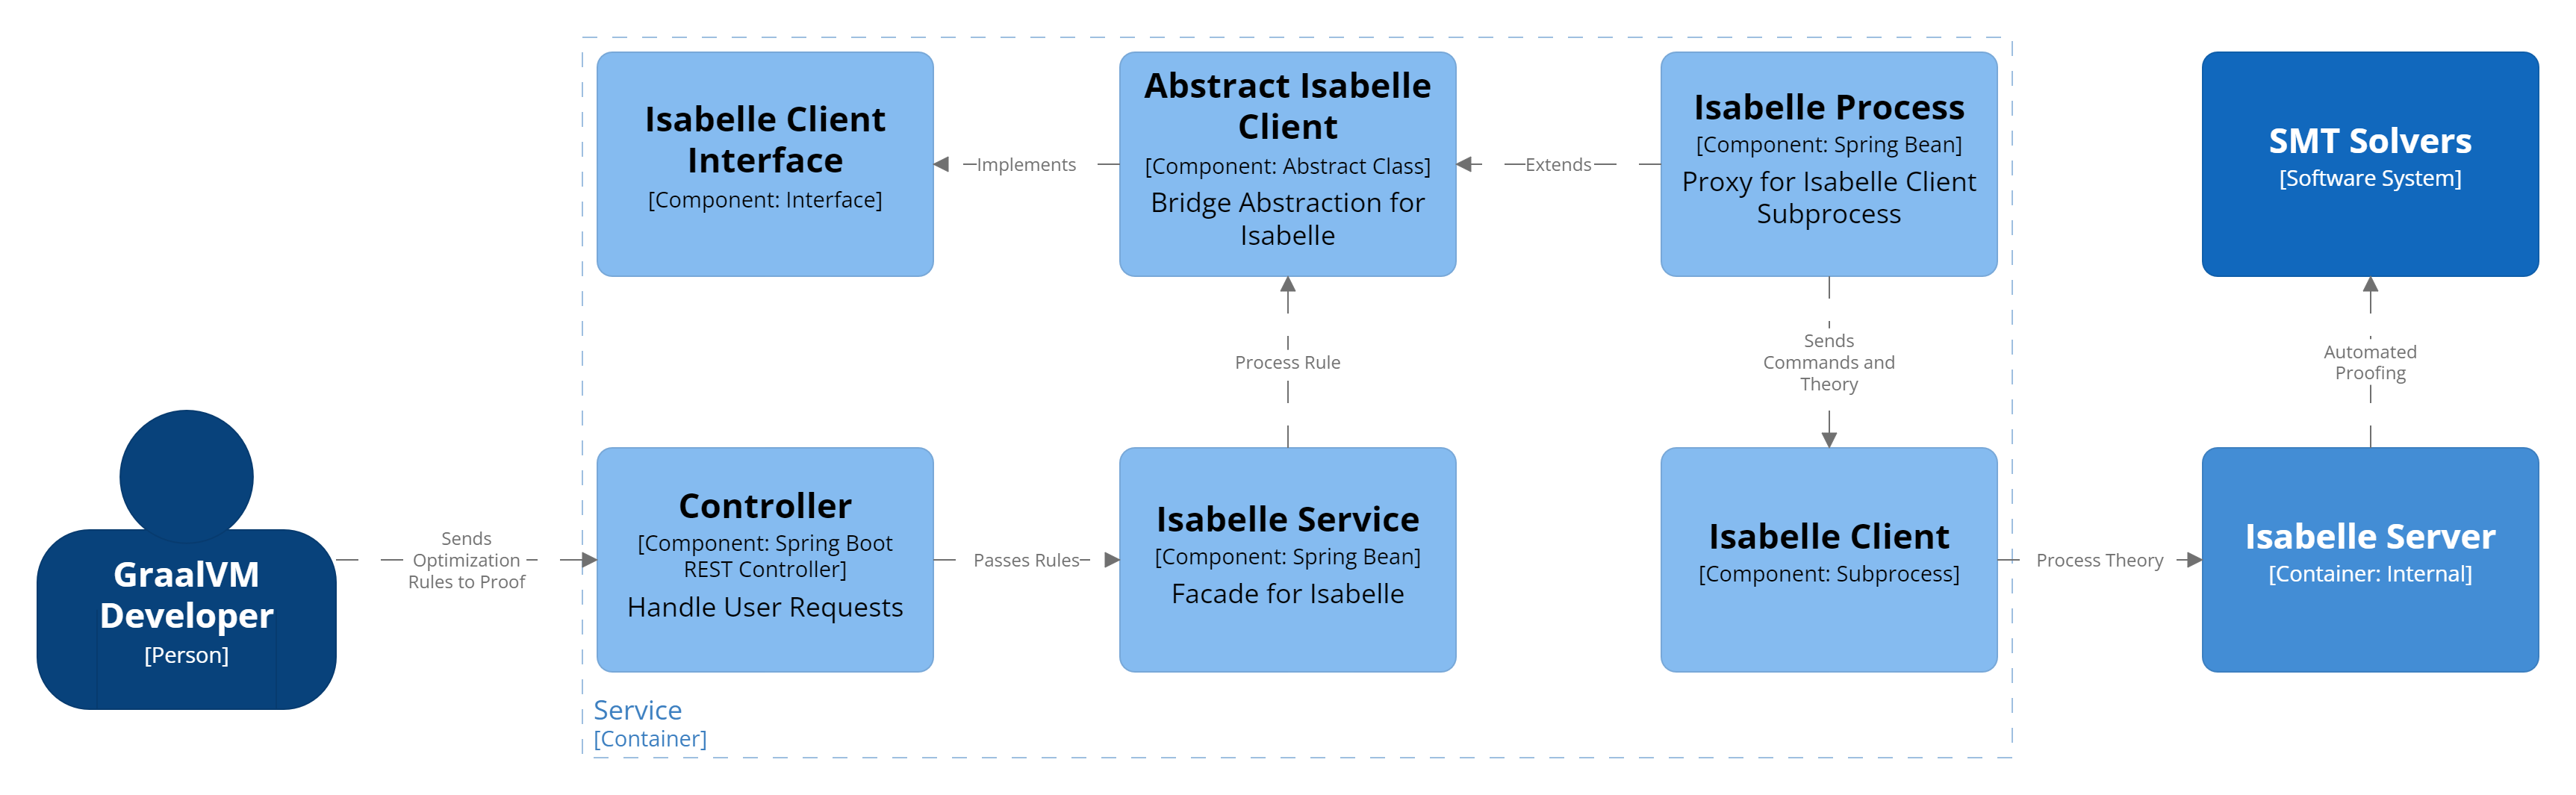
\includegraphics[width=1\textwidth]{structurizr-1-veritest_solution_1.png}
  \caption{Solution Architecture of VeriTest}
  \label{fig:architecture}
\end{figure*}

In order to provide feedback for GraalVM developers, VeriTest would need to verify whether the optimization rule:
\begin{inparaenum}
  \item is obviously false -- a counterexample exists;
  \item is obviously true -- a proof can be found;
  \item require manual proving by \emph{"proof experts"}.
\end{inparaenum}

To leverage Isabelle, VeriTest utilizes Isabelle Client - Server \cite{isabelleSystem} interactions as a method of interfacing with 
Isabelle tools. Isabelle Server acts as the core Isabelle process that allows theorems and all the required facts to 
be loaded up and processed in parallel by Isabelle/ML which is ideal for VeriTest \cite[Ch. 4.2.6]{isabelleSystem}. 
As theorems can interfere with one another, VeriTest ensures that each theorem is 
mutually exclusive by separating the sessions that they are run on, making them essentially stateless.

\cref{fig:architecture} demonstrates the architecture of VeriTest. As there are multiple ways of interacting with Isabelle Server 
\cite[Ch. 4.2]{isabelleSystem}, VeriTest abstracts the interaction by utilizing a bridge design pattern. The abstraction is implemented by 
Isabelle Process, which is a proxy for an Isabelle Client subprocess. 

Utilizing the proof tools provided by Isabelle yields a comprehensive analysis of the optimization rule, as we're making use of a battle-tested 
automated theorem prover. Passing optimization rules into Isabelle Client is done in parallel, utilizing asynchronous functions managed 
by a thread pool inside the system. In order to provide fast feedback, these asynchronous functions implements a circuit-breaker pattern 
when either a proof or a counterexample is found.

\subsection{Finding Counterexample}
\label{sec:findcounterexample}

In order to find counterexamples, we utilize Nitpick and Quickcheck from Isabelle. Optimization rules are represented as an Isabelle/HOL 
data type, the expression is fully translated into conjunctions which can be inferred as satisfiable or not \cite[Sec. 2]{Term_Graph_Optimizations}.

% Quickcheck is one of the counterexample generators in Isabelle that discover counterexamples quickly by assigning 
% free variables on the code via exhaustive test data generators \cite[Sec. 4]{isabelleProof}. Exhaustive and narrowing test data generators 
% systematically evaluates proof definitions symbolically, and generates values up to their bounds \cite[Sec. 5]{isabelleQuickcheck}.
% This is possible due to term rewriting static analysis done on proof definitions \cite[Sec. 5]{isabelleQuickcheck}.

% Nitpick is an alternative to find counterexamples for proof definitions. Instead of enumerating the bounds of free variables inside the 
% system of Isabelle, Nitpick passes conjectures into SAT solvers to search for premises that falsify the given conjectures
% \cite[Sec. 5]{isabelleProof}. If a conjecture has bounds over finite domains, Nitpick will \emph{eventually} find the counterexample.

\subsection{Finding Proof}
\label{sec:findproof}

% Sledgehammer is one of the tools in Isabelle that \emph{could} automatically prove a theorem by utilizing the inference rules and passing 
% them into resolution prover and external SMT solver to try and solve it \cite[Sec. 3]{isabelleProof}. Sledgehammer, 
% combined with external SMT solvers, can solve 60.1\% of proof goals, with a 44.7\% success rate for non-trivial goals \cite{isabelleProof}.

Sledgehammer is invoked recursively in an attempt to verify the optimization rule. As after Sledgehammer is invoked, there may be multiple 
possible proofs available, and it may not completely prove all proof obligations. Thus, we use the partially proven optimization rule and 
re-invoke Sledgehammer, until either it succeeds or fails to prove all proof obligations.

\subsection{Limitations}
\label{sec:limitations}

% Over the course of the implementation, we found a key flaw inside Isabelle Server.
Unexpectedly, there is a key flaw inside Isabelle Server.
\citet{kobschatzki_unexpected_2024} notes that Isabelle Server triggers a race condition with multiple users and sessions, unless a 
delay of several seconds is placed in between subsequent commands. Isabelle Server's source code also confirms that each command invocation 
doesn't support concurrent use. As such, this introduces a bottleneck for parallel processing of optimization rules.

\section{Evaluation}
\label{sec:evaluation}

\begin{figure}[h]
  \centering
  \begin{tabular}{llll}
    \toprule
    Result & \# Rules & Mean \pm\ \textit{SD} \\
    \midrule
    Failed & 59 & 87.06 \pm\ 49.42 \\
    Found Auto Proof & 7 & 37.73 \pm\ 3.92 \\
    Found Proof & 32 & 82.91 \pm\ 29.43 \\
    Found Counterexample & 1 & 40.79 \pm\ 4.02 \\
    Malformed & 13 & 37.96 \pm\ 4.02 \\
    No Subgoal & 2 & 37.93 \pm\ 3.38 \\
    \bottomrule
  \end{tabular}
  \caption{Evaluation of each existing Veriopt optimization rules based on runtime (in seconds)}
  \label{tab:evaluation}
\end{figure}

Evaluation is done by exporting the existing Veriopt's expression canonicalization optimization rules and iterating them five times as a benchmark on 
an AMD Ryzen 9 7900X processor with 64GB of RAM inside Windows 10 WSL environment. \cref{tab:evaluation} describes the result of the evaluation.

% Since each subsequent Isabelle command invocation is separated by the session it is run on and the bottleneck that the limitation of 
% Isabelle Server introduces, there is a baseline runtime for every verification of an optimization rule. 
Our findings suggests that there is a baseline runtime for every verification of an optimization rule, since each subsequent Isabelle command 
invocation is stateless. Additionally, the limitation of Isabelle Server introduces a bottleneck to the system.
This is demonstrated by the consistent minimum runtime of finding automatic proofs, counterexamples, and malformed rules.

The evaluated runtime suggests a significant variation of runtime for some results.
This is due to VeriTest attempting to exhaust every possible proof and counterexample for the optimization rule. 
As the complexity of optimization rules vary, the depth of the recursive tree depends on the proof obligations that 
Sledgehammer can prove. Failure to find a proof suggests that it \emph{may} be able to be proven with adequate expertise in formal proofs.

Surprisingly, some of the existing, commented out, optimization rules are malformed. After investigation, we found that it is malformed 
due to type unification errors over the IR terms.

Finally, we found that VeriTest is capable of utilizing existing lemmas inside Veriopt's current theory base to find proofs for the 
optimization rule. This implies that, as the collection of theories grow, the percentage of optimization rules that can be 
automatically proven is improved.

% % regular IEEE prefers the singular form
% \section*{Acknowledgment}

% Identification of funding sources and other support, and thanks to individuals and groups that assisted in the 
% research and the preparation of the work should be included in an acknowledgment section, which is placed just before 
% the reference section in your document.

%%% ===============================================================================
%%% Bibliography
%%% ===============================================================================

% trigger a \newpage just before the given reference
% number - used to balance the columns on the last page
% adjust value as needed - may need to be readjusted if
% the document is modified later
%\IEEEtriggeratref{8}
% The "triggered" command can be changed if desired:
%\IEEEtriggercmd{\enlargethispage{-5in}}

% Enable to reduce spacing between bibitems (source: https://tex.stackexchange.com/a/25774)
% \def\IEEEbibitemsep{0pt plus .5pt}

\bibliographystyle{IEEEtranN} % IEEEtranN is the natbib compatible bst file
% argument is your BibTeX string definitions and bibliography database(s)
\bibliography{isabelle,veriopt,references}
%

\end{document}
